\documentclass[10pt,a5paper,twoside]{book}
\usepackage[utf8]{inputenc}
\usepackage[czech]{babel}
\usepackage[T1]{fontenc}
\usepackage{amsmath}
\usepackage{amsfonts}
\usepackage{amssymb}
\usepackage{hyperref}
\usepackage{wrapfig}
\usepackage[dvips]{graphicx}
\usepackage[top=1.5cm, left=1.2cm, bottom=1.0cm, includefoot]{geometry}
\usepackage{eso-pic}
\usepackage{pdfpages}
\usepackage{textpos}
\usepackage{titlesec}
\usepackage{verbatim}
\usepackage{multicol}

\fontencoding{T1}
\fontfamily{cmss}
\fontseries{m}
\fontshape{n}
\setlength{\belowcaptionskip}{-15pt} % mezera za popiskem obrázku
\usepackage{xcolor}
\usepackage{pdfpages}
% pdftk TitlePage14_1.pdf Jihacas14_1.pdf cat output Jihocas_14_1-WEB_kontrola.pdf spojeni pdf

\titleformat{\section}
{\color{black}\normalfont\Large\bfseries}
{\color{black}\thesection}{1.2em}{}

\newcommand{\autor}[1]{
	\begin{flushright}
	\textit{#1}
	\end{flushright}
}

\begin{document} 

%\begin{titlepage}
\begin{center}

% Upper part of the page. The '~' is needed because \\
% only works if a paragraph has started.
\includegraphics[width=0.15\textwidth]{./logo}~\\[1cm]

\textsc{\LARGE University of Beer}\\[1.5cm]

\textsc{\Large Final year project}\\[0.5cm]

% Title
\HRule \\[0.4cm]
{ \huge \bfseries Lager brewing techniques \\[0.4cm] }

\HRule \\[1.5cm]

% Author and supervisor
\begin{minipage}{0.4\textwidth}
\begin{flushleft} \large
\emph{Author:}\\
John \textsc{Smith}
\end{flushleft}
\end{minipage}
\begin{minipage}{0.4\textwidth}
\begin{flushright} \large
\emph{Supervisor:} \\
Dr.~Mark \textsc{Brown}
\end{flushright}
\end{minipage}

\vfill

% Bottom of the page
{\large \today}

\end{center}
\end{titlepage}



\section*{K obrázku na titulní straně}
Obraz od našeho nového člena Vladana Špačka. Obraz je ze série Poselství duhy a originál je olejomalba o rozměrech 1,5 X 2 m.
Pan Špaček se kromě malování zabývá radioastronomií. Vlastní radioteleskop na 12 GHz, pomocí kterého pravidelně měří aktivitu Slunce.

\vfill
\section*{JihoČAS}
Vydává: Jihočeská pobočka České astronomické společnosti.\\
Redakce a adresa pro zasílání příspěvků: \textbf{Martin Kákona}, U Jatek 19/III, 392 01 Soběslav, e-mail: \href{mailto:martin.kakona@astro.cz}{martin.kakona@astro.cz}.\\
Sazba: \textbf{Roman Dvořák}, e-mail: \href{mailto:roman-dvorak@email.cz}{roman-dvorak@email.cz}.\newpage
\null
\vfill

\section*{Členské příspěvky}

Členské příspěvky posílejte na účet \textbf{2900452466/2010}. Členské příspěvky na příští rok pošlete nejpozději do konce října! Tento termín je nutné dodržet, jinak nedostanete členskou průkazku vloženu do Astropisu. Členské příspěvky na příští rok jsou 600 Kč (450 Kč studenti a důchodci). Z této částky odvádí pobočka 500 Kč resp. 400Kč do Prahy (hradí se z ní například náklady na tisk Astropisu) a 100 Kč (50 Kč) si nechává pobočka (to použijeme jako spolufinancování dotace RVS). Do zprávy pro příjemce prosím napište své jméno. Zda platba došla, si můžete ověřit zde: \href{https://www.fio.cz/ib2/transparent?a=2900452466}{www.fio.cz/ib2/transparent?a=2900452466}.

\section*{Výroční schůze}

Letošní členská schůze se uskuteční mimo pořadí na hvězdárně Františka Nušla v Jindřichově Hradci v sobotu 19. listopadu od 15 hodin. Letos nás čekají volby, tak si prosím promyslete, kdo budete chtít pracovat ve výboru pobočky a co si vezmete na starost. 

Tady je krátký seznam toho, co je nutné dělat:

\begin{itemize}
  \setlength\itemsep{-1.7mm}
\item Vedení členské evidence.
\item Tvorba a synchronizace členské databáze.
\item Vybírání členských příspěvků.
\item Evidence členských příspěvků v členské databázi ČAS.
\item Vedení účetní knihy (elektronicky).
\item Administrace a tvorba webu pobočky.
\item Sazba JihoČASu.
\item Jazyková korektura JihoČASu.
\item Tisk JihoČASu.
\item Vazba JihoČASu.
\item Tisk obálek a Rozesílání JihoČASu.
\item Jednou za rok účast na „malém setkání složek“ ČAS.
\item Jednou za rok účast na „velkém setkání složek“ nebo sjezdu ČAS.
\item Jednou za rok vyúčtování dotace.
\item Vymáhání členských příspěvků od neplatičů (po 15. 11. do konce roku).
\item Sestavení ročního plánu práce pobočky (do 15. 9.).
\item Sepsání žádosti o dotaci na kalendářní rok (do 15. 9.).
\item Sestavení rozpočtu pobočky na kalendářní rok (do 15. 9.).
\item Sepsání výroční zprávy (do 15. 1.).
\item Vyplnění formuláře RVS o aktivitách za uplynulý rok (do 15. 1.).
\item Organizace společného pozorování.
\item A v neposlední řadě vymýšlení náplně práce pobočky.
\end{itemize}






\newpage
\section*{Hvězdárna na 15. poledníku chystá změny ...}
\autor{Mgr. Jana Jirků \\ Hvězdárna F. Nušla, Jindřichův Hradec}

\begin{wrapfigure}{r}{0.5\textwidth}
  \begin{center}
    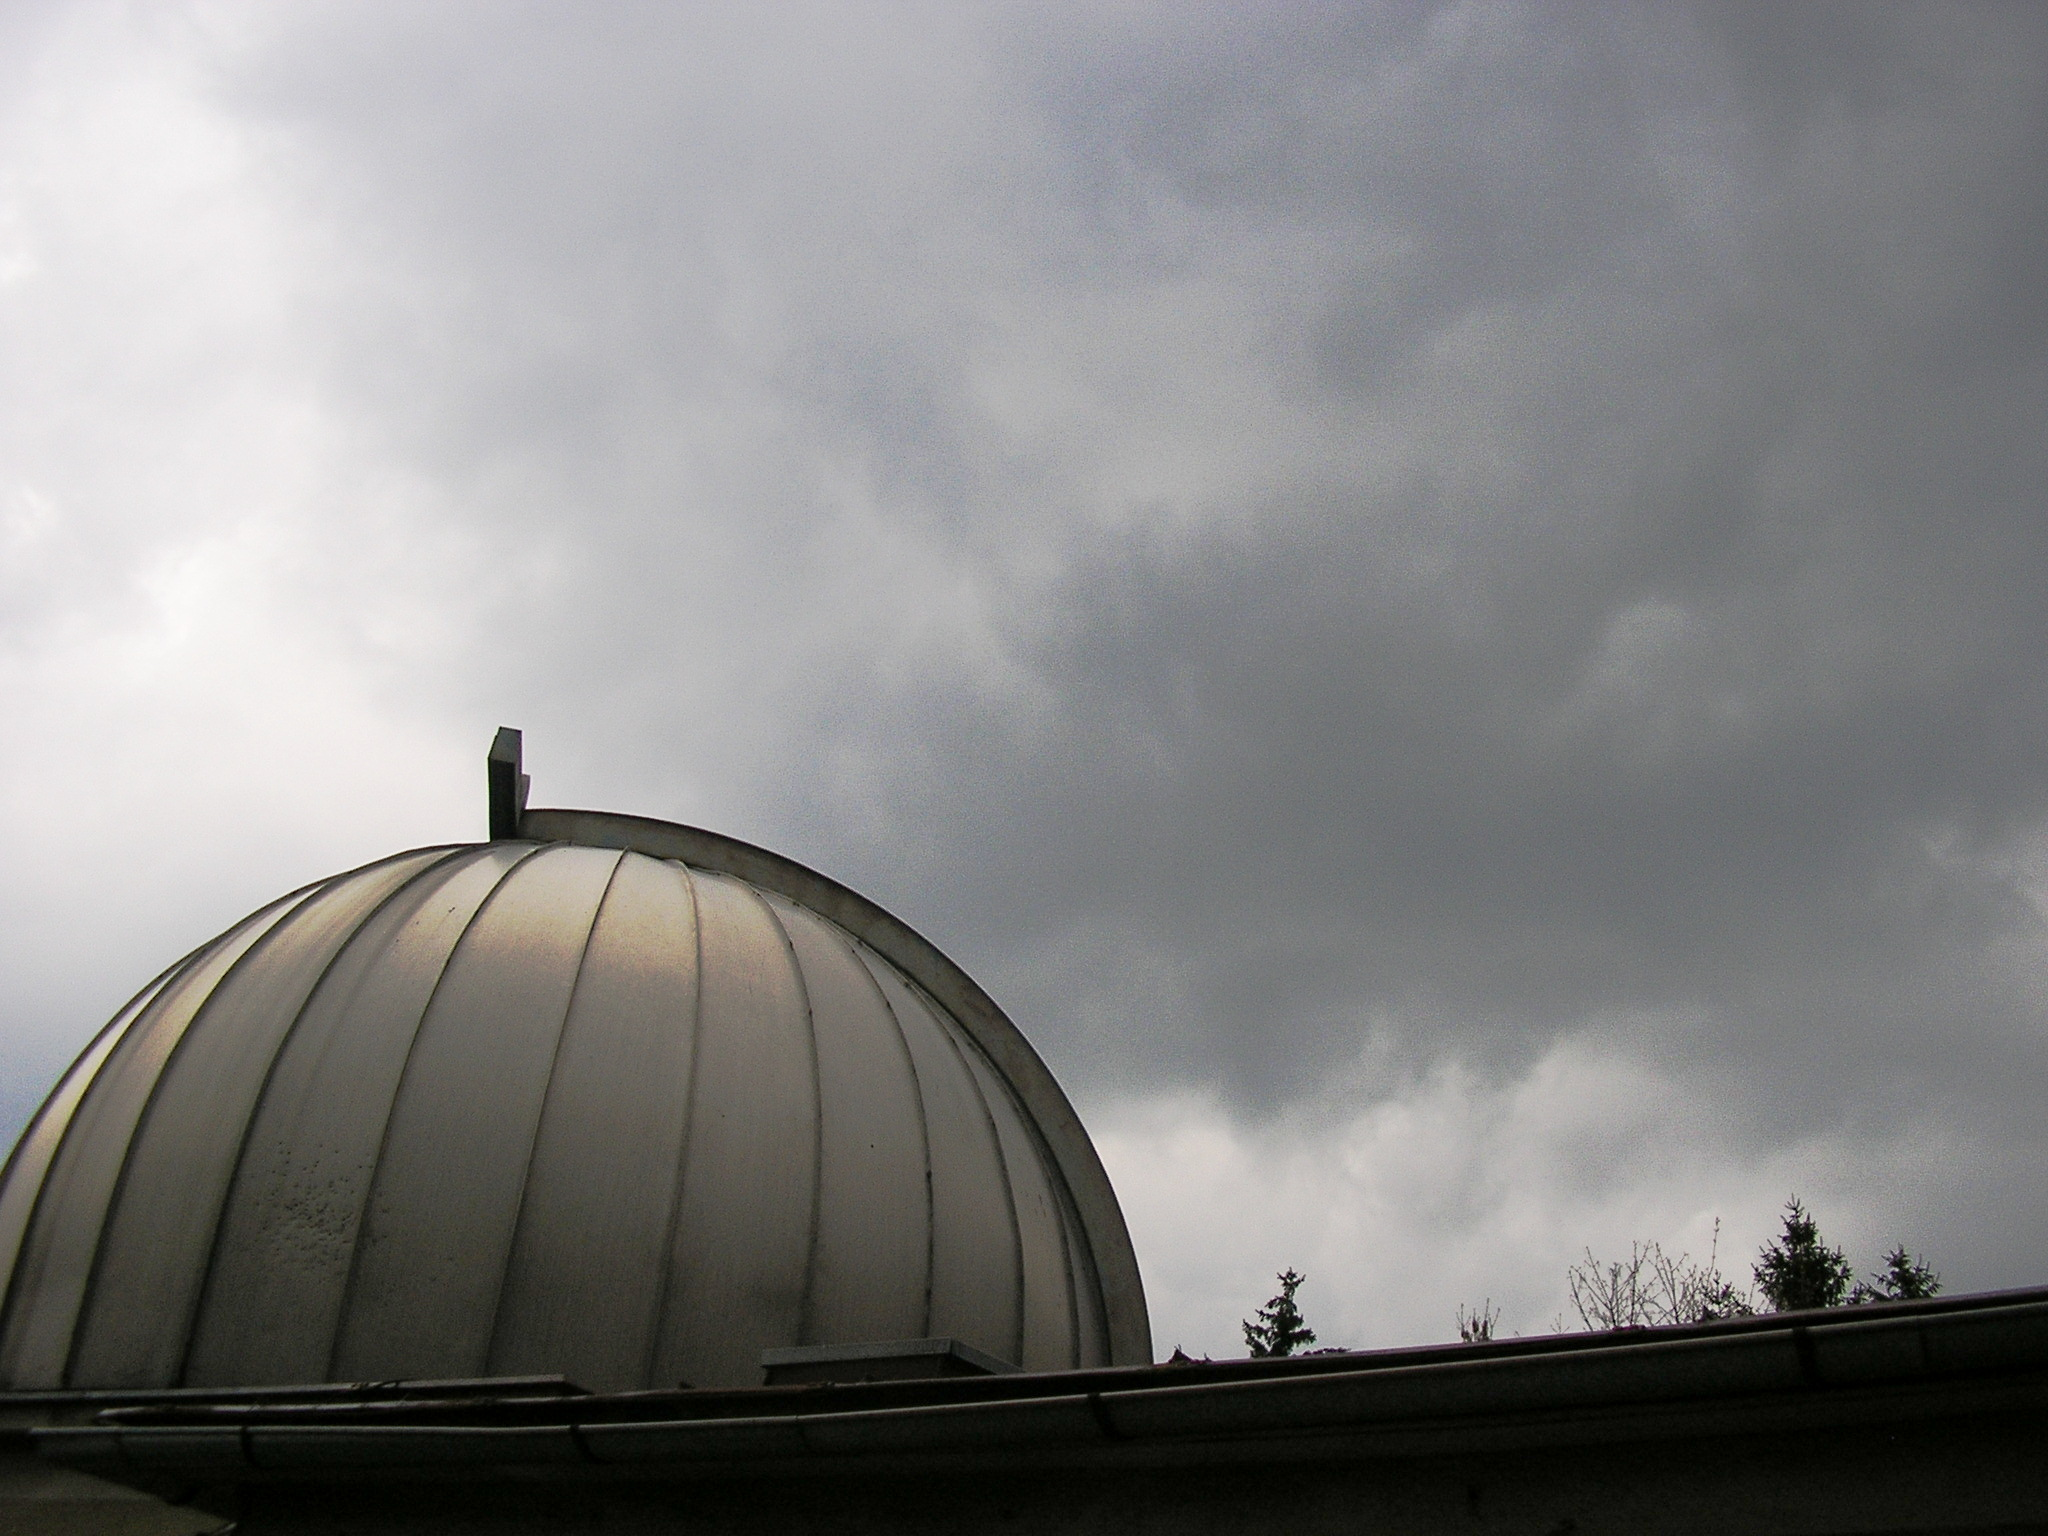
\includegraphics[width=0.5\textwidth]{bourka.JPG}
  \end{center}
\end{wrapfigure}

Jak již mnozí jistě víte, Hvězdárna F. Nušla nyní stojí před významnou událostí, kterou je možná docela velká rekonstrukce. Kdo u nás byl, jistě si řekne, že to opravdu už bylo zapotřebí.
Máme velmi malý projekční sálek, který pojme sotva jednu školní třídu, proto přednášky, akce pro děti i veřejnost, či společenské večery s astronomií a další akce musíme pořádat v takto stísněném prostředí ve velkém diskomfortu všech zúčastněných. Nemáme prostory pro skladování zařízení, nemáme kuchyňku, kde by bylo možné nějak kulturně umýt nějaký ten hrnek nebo talíř. Voda je zavedená pouze na WC, což je jediné místo, kde si každý umyje svůj hrnek od kafe. Nemáme ani šatnu pro děti ze škol, kterých chodí na naše programy k výuce opravdu dost.

Původně nám šlo o to, abychom přesvědčili vedení našeho města, že je třeba zvětšit přednáškové prostory, vyznačit  15. poledník, který prochází kousek před budovou a také nějak opravit nebo upravit přístup k budově Hvězdárny. Totiž velmi vzrostlé smrky, hlavně kolem východního plotu hvězdárenské zahrady, na skalnatém podloží, nemají se stále se zvětšujícím kořenovým systémem jinou možnost, než vystupovat nad povrch. To v trávníku, byť udržovaném, působí návštěvníkům a vlastně i nám značné problémy se pohybovat bezpečně kolem budovy Hvězdárny, zejména potmě.

Samozřejmě jsme mysleli i na naše handicapované spoluobčany, kteří mají sice v současné době možnost podívat se na oblohu velkým přístrojem z nějakého stanoviště na zahradě před budovou, ale na pozorovací terasy, ani do kopule bohužel nemají přístup.

Když už jsem zmínila pozorovací terasy, máme vlastně dvě; jednu na jih budovy a druhou na sever. Jižní terasa je velmi dobré pozorovací místo a rádi bychom ji viděli ještě vylepšenou o odsuvnou střechu, aby zde mohly zůstávat nastálo alespoň stativy, možná i nějaký dalekohled. To teď není možné, vzhledem k vysoké pravděpodobnosti nebezpečí napadení nejrůznějšími kriminálními živly. Takže dalekohledy i stativy přinášíme a odnášíme a skladujeme na velmi malém prostoru v horním vestibulu. Návštěvníci, jdoucí pozorovat na jižní terasu jsou nuceni kolem nich procházet dosti úzkým místem, proto nelze vyloučit ani riziko poranění nebo poškození majetku. 

\begin{wrapfigure}{r}{0.6\textwidth}
  \begin{center}
    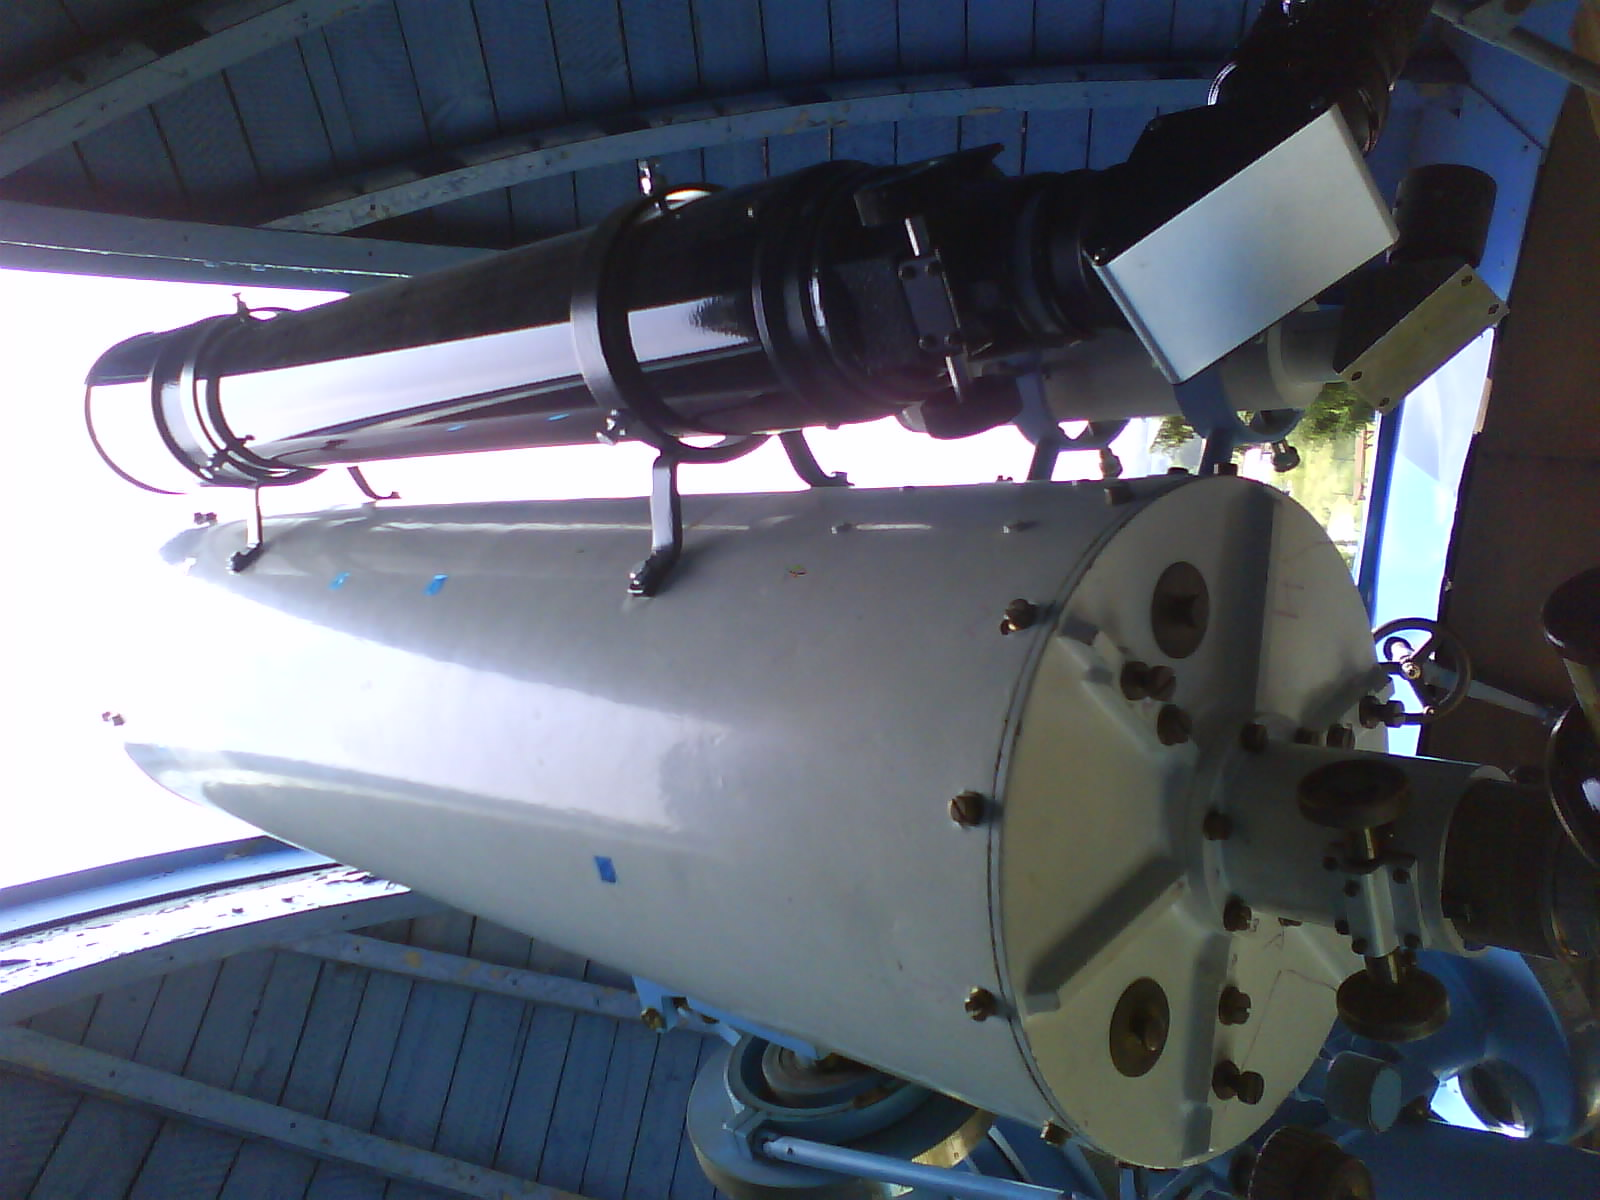
\includegraphics[width=0.58\textwidth]{starasestava.JPG}
  \end{center}
\end{wrapfigure}

Severní terasa je ale k nočnímu pozorování nepoužitelná, a tak zcela zbytečná. Je nasměrovaná k městu, kde doslova pár metrů od příjezdové cesty do areálu máme panelákové sídliště a s tím i spoustu světel. Toto bychom viděli jako další místo pro změnu; z nepotřebné terasy by mohla vzniknout klubovna, například pro zájmové kroužky a další akce s dětmi, co pořádáme. Doposud vlastně k veškerému dění na Hvězdárně sloužil a slouží pouze zmíněný malý sálek a to rozhodně nestačí, nehledě na to, že nelze podniknout třeba dvě akce najednou.  

V neposlední řadě by se hodila i malá dílnička, kde by se dalo ledasco opravit, upravit, vyčistit atd. 

Tento "vlak událostí" se dal do pohybu po jednom Předvánočním posezení, které pravidelně pořádáme už více než 10 let a zveme kromě významných hostů z oboru astronomie i členy jindřichohradeckého zastupitelstva a úředníky MÚ. V posledních letech a zvyšujícím se počtu zúčastněných bylo nasnadě, že situace je kritická.

Nyní čekáme na dokončení projektu, schválení rozsahu změn a další rozhodnutí. Také jsme přišli na to, jak popř. zvětšit i prostory kopule, ale o tom bych se zatím nerada rozšiřovala, to je ještě skutečně ve hvězdách :).

Můžeme jen slíbit, že až bude rozhodnuto a "uvaříno", podělíme se s Vámi všemi moc rádi o všechny novinky.
	
\section*{Vnučka Kozelská}
\autor{Mgr. Jana Jirků \\ Hvězdárna F. Nušla, Jindřichův Hradec}
Naše Hvězdárna každoročně nejen v létě uvítá mnoho návštěvníků, exkurzí, hromadných i jiných specifických návštěv. Počet zúčastněných lidí bývá různý, někdy – a skoro většinou - přesahující kapacitu našeho malého projekčního sálku. (Mimo to pořádáme i výjezdy na letní tábory s přednáškami a dalekohledy za účelem pozorování -  exkurzisti, kteří nás navštěvují, bývají jak z blízka, tak  často z poměrně velké, až značné vzdálenosti a i my jezdíme na táborové přednášky do vzdálenosti až kolem 100 km od JH). 

Letošní léto se ale stalo cosi ojedinělého, o čem rozhodně nelze říct, že je běžné ...
...Takhle jako vždy a normálně jsme se sešli na Hvězdárně, protože jsme měli objednanou exkurzi z Dlouhé Brtnice na Jihlavsku. 

Objednaná exkurze měla čítat skoro čtyřicet osob. To je běžné. Ale protože, jak skoro asi všichni dobře víte, máme v JH fakt malý projekční sálek, musíme řešit tyto exkurze tak, že skupinu rozdělíme na dvě části: první jde nejdříve do kopule na pozorování, druhá do projekčního sálku na přednášku a promítání. Po určité době, jak je domluveno předem podle časových možností návštěvníků, se skupiny vymění a tak obě absolvují  plný náš nabízený program.

Ale abych se konečně dostala k „jádru mezka“: ze skupiny z Brtnice najednou vystoupila paní s hláškou: „jéé, to je děda!“ Bez dalších průtahů jsme se dozvěděli, že je vnučkou tvůrce naší montáže, pana Františka Kozelského, dcera jeho dcery. 

Takže se opět potvrdilo rčení, „jak je ten svět malej“, prostě jeden čumí, co vše se může stát :)!!! Paní  nás navštívila i s vnoučaty a souhlasila s fotografováním, takže snímky přikládám.

\begin{figure}[!htbp]
	\begin{center}
  		\includegraphics*[width=11.5cm]{kozelsti.jpg}
  	\end{center}
\end{figure}


\section*{Hvězdárna Františka Pešty v Sezimově Ústí \\- 50. let}

Dne 10. 10. 2015 připravili členové Hvězdárny Františka Pešty v Sezimově Ústí rozsáhlou oslavu 50. výročí otevření své observatoře. Jak nás hned v úvodu upozornil dlouholetý vedoucí hvězdárny Petr Bartoš, datum oslav nebylo vybráno náhodně. Ale zcela v duchu cimrmanovské poučky, že důležité historické milníky se mají odehrávat ve snadno zapamatovatelných časových okamžicích. Ke skutečnému otevření sezimovské hvězdárny došlo o něco dříve, shodou okolností i toto datum naplňuje zmíněnou tezi: stalo se tak 6. 6. 1965. 

Hosté byli přivítáni výstavou z dílny astronomického kroužku (lineární urychlovač částic), bohatým občerstvením a především poutavou přednáškou Petra Bartoše o historii hvězdárny. Ve své prezentaci měl z čeho vybírat - k tomuto výročí totiž napsal výpravnou publikaci \textit{Astronomie v Sezimově Ústí a František Pešta}, kterou v rámci oslav pokřtil tehdejší předseda závodního výboru a organizátor stavebních prací pan Václav Kalina.

Hvězdárna Františka Pešty v Sezimově Ústí spadá rokem vzniku do druhé poválečné vlny výstavby lidových (veřejných) hvězdáren.  Ve společnosti byla silná poptávka po astronomickém poznání vyvolaném zejména úspěchy kosmonautiky a tak mnohé žádosti astronomických nadšenců o finanční dotaci na stavbu hvězdárny padly na úrodnou půdu. Vybudovat novou hvězdárnu bylo tehdy možné pouze pod patronátem tzv. závodních výborů jednotlivých státních podniků.

Nápad, projekt, organizace výstavby, zajištění stavebního personálu a mnohdy i potřebné vybavení včetně hlavního dalekohledu však téměř bez výjimky ležely na bedrech toho, kdo s nápadem nové hvězdárny přišel. Od dob steplingových se mnoho nezměnilo. A jak mi řekl pan Václav Kalina: \textit{„Při objednávání stavebních prací a jejich fakturaci jsem stál pořád jednou nohou v kriminále. Mohl jsem vyplatit maximálně 8 Kčs za hodinu práce. Ale takového řemeslníka byste v Čechách nenašel. Minimum bylo dvacet, v opačném případě se s vámi nikdo nebavil. Tak jsem musel sehnat přátele, na které jsem ten rozdíl mohl napsat. Jinak by nic nebylo.”}

Být zakladatelem hvězdárny znamenalo i v roce 1965 zvládnout mnoho profesí najednou: od mediátora přesvědčujícího svého zaměstnavatele k nemalé investici, přes stavbyvedoucího, prosebníka svých přátel o práci zdarma až po vedoucího nové hvězdárny, který ji vymýšlel měsíční program a zajišťoval pravidelnou činnost. Bez nároku na honorář a obvykle jen ve svém volném čase. Právem se tedy jména zakladatelů v několika případech stala součástí názvu jimi vybudovaných hvězdáren jako poděkování za veliké úsilí vynaložené při vzniku a provozu v prvních letech činnosti. A nejinak je tomu i v případě Hvězdárny Františka Pešty v Sezimově Ústí.   

V pokročilém odpoledni se program oslav přenesl do nedalekého kinosálu, kde na účastníky oslav čekaly tři zajímavé výstavy - Astronomie v Sezimově Ústí, Strkovské meteority a Poezie vesmíru. Vrcholem oslav se pak stal triptych úchvatných astronomických přednášek Jiřího Grygara (Knihy a hvězdy), Pavla Spurného (Bolidy a pády meteoritů) a Petra Horálka (Lovy skvostů temné oblohy).    







\begin{figure}[!htbp]
	\begin{center}
  		\includegraphics*[width=10cm]{jg.jpg}
  	\end{center}
Jiří Grygar zahajuje oslavy 50. výročí vzniku Hvězdárny Františka Pešty
\end{figure}



\section*{Graf, který byste měli vidět}
\autor{Martin Kákona}

V grafu je uvedeno zastoupení jader, které k nám přilétají z kosmu. Na logaritmické ose je vynesen počet jader na sto jader křemíku. Graf končí niklem, ale přilétají k nám prakticky všechny relativně stabilní prvky, které to od času svého vzniku k nám stihnou, takže na sto miliónů atomů křemíku připadne jeden atom uranu.



\begin{figure}[!htbp]
	\begin{center}
  		\includegraphics*[width=9cm]{abs_cr_sol.png}
  	\end{center}
\end{figure}














%\begin{figure}[htbp]
% \centering
%  \includegraphics*[width=10cm]{moon.jpg}
%\end{figure}
%\begin{figure}[htbp]
% \centering
%  \includegraphics*[width=10cm]{JH/moon.eps}
%\end{figure}




\end{document}
 
 
%	\begin{itemize}
%	\item 
%	\end{itemize}
